\section{Advanced feature}
In the evaluation section ~\ref{sec:eval}, we have seen that training the model takes a lot of time while inference is fast. To overcome this problem, we tried some advance feature such as (1) Inference with previously saved model (2) Save and load model

\subsection{Inference with previously saved model}
\label{sec:appIO}
We can train the model with SPML+privacy in native mode (without Intel SGX and SCONE). In this mode, training time is very less (around 30 seconds) for the MNIST dataset as compare to SPML+privacy+security mode (around 775 seconds), which will save a lot of the time. The model which we have got can be used for doing inference in SCONE hardware mode with security property enabled. We ran some measurements wherein we use the model trained in native mode and deploy the model in SCONE hardware mode to check the impact. As seen in the Figure  ~\ref{fig:appendixPSMnistAccuracyInference} and ~\ref{fig:appendixPSMnistLatencyInference}, the accuracy and latency remains almost same as compare to native mode ~\ref{fig:appendixnativeMnistAccuracyInference} and ~\ref{fig:appendixnativeMnistLatencyInference} and the hardware mode ~\ref{fig:appendixhwMnistAccuracyInference} and ~\ref{fig:appendixhwMnistLatencyInference}.

\subsection{Save and load model}
\label{sec:appNHmode}
We can train the model with some samples in SPML+privacy in native mode (without Intel SGX and SCONE) and later load the saved model and continue training in hardware mode. This type of technique is used in federated learning also where in each individual device train models using local data in a decentralized way, and then send this trained model to central server which combines resultant model to generate a global model. We can opt for such approach to reduce training time.
As seen in the Figure ~\ref{fig:appendixFLMnistAccuracyInference},  ~\ref{fig:appendixFLMnistLatencyInference} the accuracy and latency remains almost same as compare to native ~\ref{fig:appendixnativeMnistAccuracyInference} and ~\ref{fig:appendixnativeMnistLatencyInference}, and the hardware mode ~\ref{fig:appendixhwMnistAccuracyInference} and ~\ref{fig:appendixhwMnistLatencyInference}

\begin{figure}
     \begin{subfigure}{0.5\textwidth}
         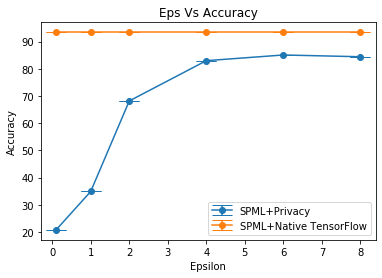
\includegraphics[width=\textwidth]{images/Inference/MnistNativeAccuracyInference.png}
         \caption{Accuracy}
         \label{fig:appendixnativeMnistAccuracyInference}
     \end{subfigure}
     \begin{subfigure}{0.5\textwidth}
         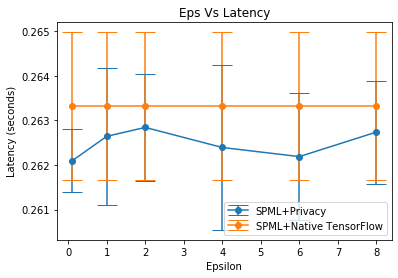
\includegraphics[width=\textwidth]{images/Inference/MnistNativeLatencyInference.png}
         \caption{Latency}
         \label{fig:appendixnativeMnistLatencyInference}
     \end{subfigure}
        \caption{MNIST Dataset - Inference - Native mode without Intel SGX and SCONE}
     \begin{subfigure}{0.5\textwidth}
         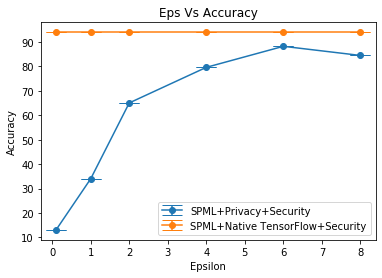
\includegraphics[width=\textwidth]{images/Inference/MnistHwAccuracyInference.png}
         \caption{Accuracy}
         \label{fig:appendixhwMnistAccuracyInference}
     \end{subfigure}
     \begin{subfigure}{0.5\textwidth}
         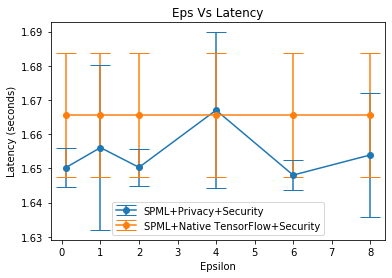
\includegraphics[width=\textwidth]{images/Inference/MnistHwLatencyInference.png}
         \caption{Latency}
         \label{fig:appendixhwMnistLatencyInference}
     \end{subfigure}
        \caption{MNIST Dataset - Inference - Hardware mode with Intel SGX and SCONE}
     \begin{subfigure}{0.5\textwidth}
         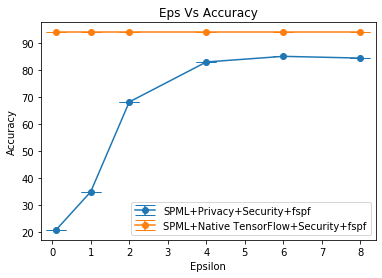
\includegraphics[width=\textwidth]{images/Inference/MnistPSAccuracyInference.png}
         \caption{Accuracy}
         \label{fig:appendixPSMnistAccuracyInference}
     \end{subfigure}
     \begin{subfigure}{0.5\textwidth}
         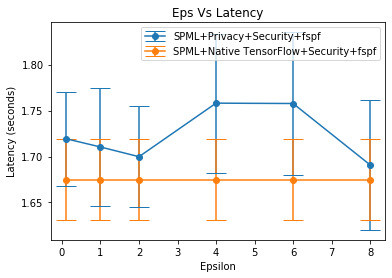
\includegraphics[width=\textwidth]{images/Inference/MnistPSLatencyInference.png}
         \caption{Latency}
         \label{fig:appendixPSMnistLatencyInference}
     \end{subfigure}
        \caption{MNIST Dataset - Inference+Saved Model - Hardware mode + Fspf with Intel SGX and SCONE}
\end{figure}


\begin{figure}
     \begin{subfigure}{0.5\textwidth}
         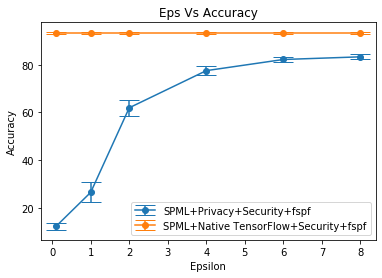
\includegraphics[width=\textwidth]{images/Training/MnistFLAccuracy.png}
         \caption{Accuracy}
         \label{fig:appendixFLMnistAccuracyTraining}
     \end{subfigure}
     \begin{subfigure}{0.5\textwidth}
         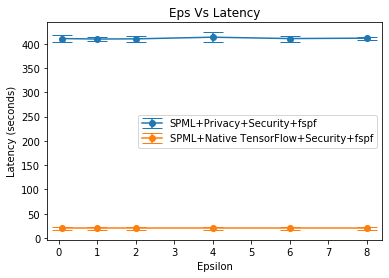
\includegraphics[width=\textwidth]{images/Training/MnistFLLatency.png}
         \caption{Latency}
         \label{fig:appendixFLMnistLatencyTraining}
     \end{subfigure}
        \caption{MNIST Dataset - training - native+hardware Mode - Hardware mode + Fspf with Intel SGX and SCONE}
     \begin{subfigure}{0.5\textwidth}
         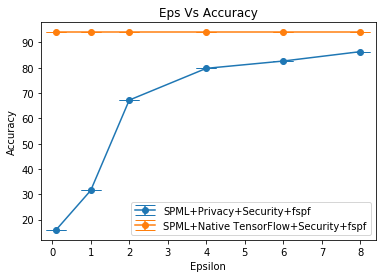
\includegraphics[width=\textwidth]{images/Inference/MnistFLAccuracyInference.png}
         \caption{Accuracy}
         \label{fig:appendixFLMnistAccuracyInference}
     \end{subfigure}
     \begin{subfigure}{0.5\textwidth}
         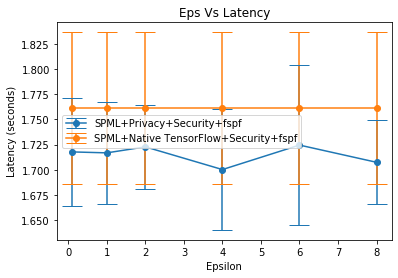
\includegraphics[width=\textwidth]{images/Inference/MnistFLLatencyInference.png}
         \caption{Latency}
         \label{fig:appendixFLMnistLatencyInference}
     \end{subfigure}
        \caption{MNIST Dataset - inference - native+hardware Mode - Hardware mode + Fspf with Intel SGX and SCONE}
\end{figure}

